
\chapter{Grundlagen}
\thispagestyle{fancy}

\section{Bandstruktur von Gruppe-III Nitriden}

Die wichtige Gruppe der III-Nitridhalbleiter setzt sich aus den Metallen
der dritten Hauptgruppe Aluminium (Al), Gallium (Ga) und Indium (In) zusammen.
Der Schwerpunkt dieser Arbeit liegt auf dem AlGaN-Materialsystem mit hohen Al-Konzentration. Das Mischverhältnis bestimmt hierbei die Bandlückenergie des Verbindungshalbleiters. Durch die unterschiedlichen Bandlückenergien von Aluminium mit 6.03 eV~\cite{fenaln} und GaN mit 3.4 eV~\cite{pipr} eignet sich AlGaN besonders für die Emission im Wellenlängenbereich von UV-A bis UV-C. 
Die Bandlückenenergie von AlGaN lässt sich durch Interpolation der binären Energien von GaN und AlN in Abhängigkeit des Kompositionsverhältnisses x berechnen, wobei ein zusätzlicher Bowing-Parameter für die nichtlineare Abweichung hinzugefügt wird. 

\begin{equation}
    E_{Al_{x}Ga{1-x}N} = E_{AlN} \cdot x + E_{GaN} \cdot (1-x) - b_{AlGaN} \cdot x \cdot (1-x) 
\end{equation}


\newpage
\section{Polarisationsfeld und QCSE in III/V Halbleitern}

Die Gruppe der III-Nitrid-Halbleiter kristallisiert in der Wurtzitstruktur. Anschaulich bedeutet dies, dass ausgehend von der hexagonal dichtesten Kugelpackung in Doppellagen, die Gruppe-III-Metallen und Stickstoff (N) sich entlang der c-Achse in der Abfolge A-B-A-B anordnen~\cite{buchc} wie in Abb. 2.1 dargestellt ist. 
\newline
Aufgrund der fehlenden Inversionssymmetrie und stark unterschiedlichen Elektronegativitäten des Stickstoffs und der entsprechenden Gruppe III-Metalle bilden sich Polarisationsfelder aus, die entlang der auf der Basalebende stehenden c-Achse verlaufen. Hier unterscheidet man zwischen zwei Arten von Polarisationsfeldern, die spontane Polarisation $ \vec{P}^{sp} $ und die piezoelektrische Polarisation $ \vec{P}^{pz} $.
\newline\newline
Die spontante Polarisation entsteht durch Dipolmomente im Kristall die sich aufgrund von ungleichen Bindungslängen nicht komplett aufheben. Ursprung der 
Dipolmomente im AlGaN sind die unterschiedlichen Elektronegativitäten zwischen den III-V Elementen und bedingt durch die angestrebte Minimierung der Gesamtenergie, kommt es zur Abweichung vom idealen Tetraederwinkel von $109,5^{\circ}$ ~\cite{ambacher2002}.
%
\begin{figure}[htb]
    \centering
    \begin{minipage}[t]{0.49\linewidth}
        \centering
        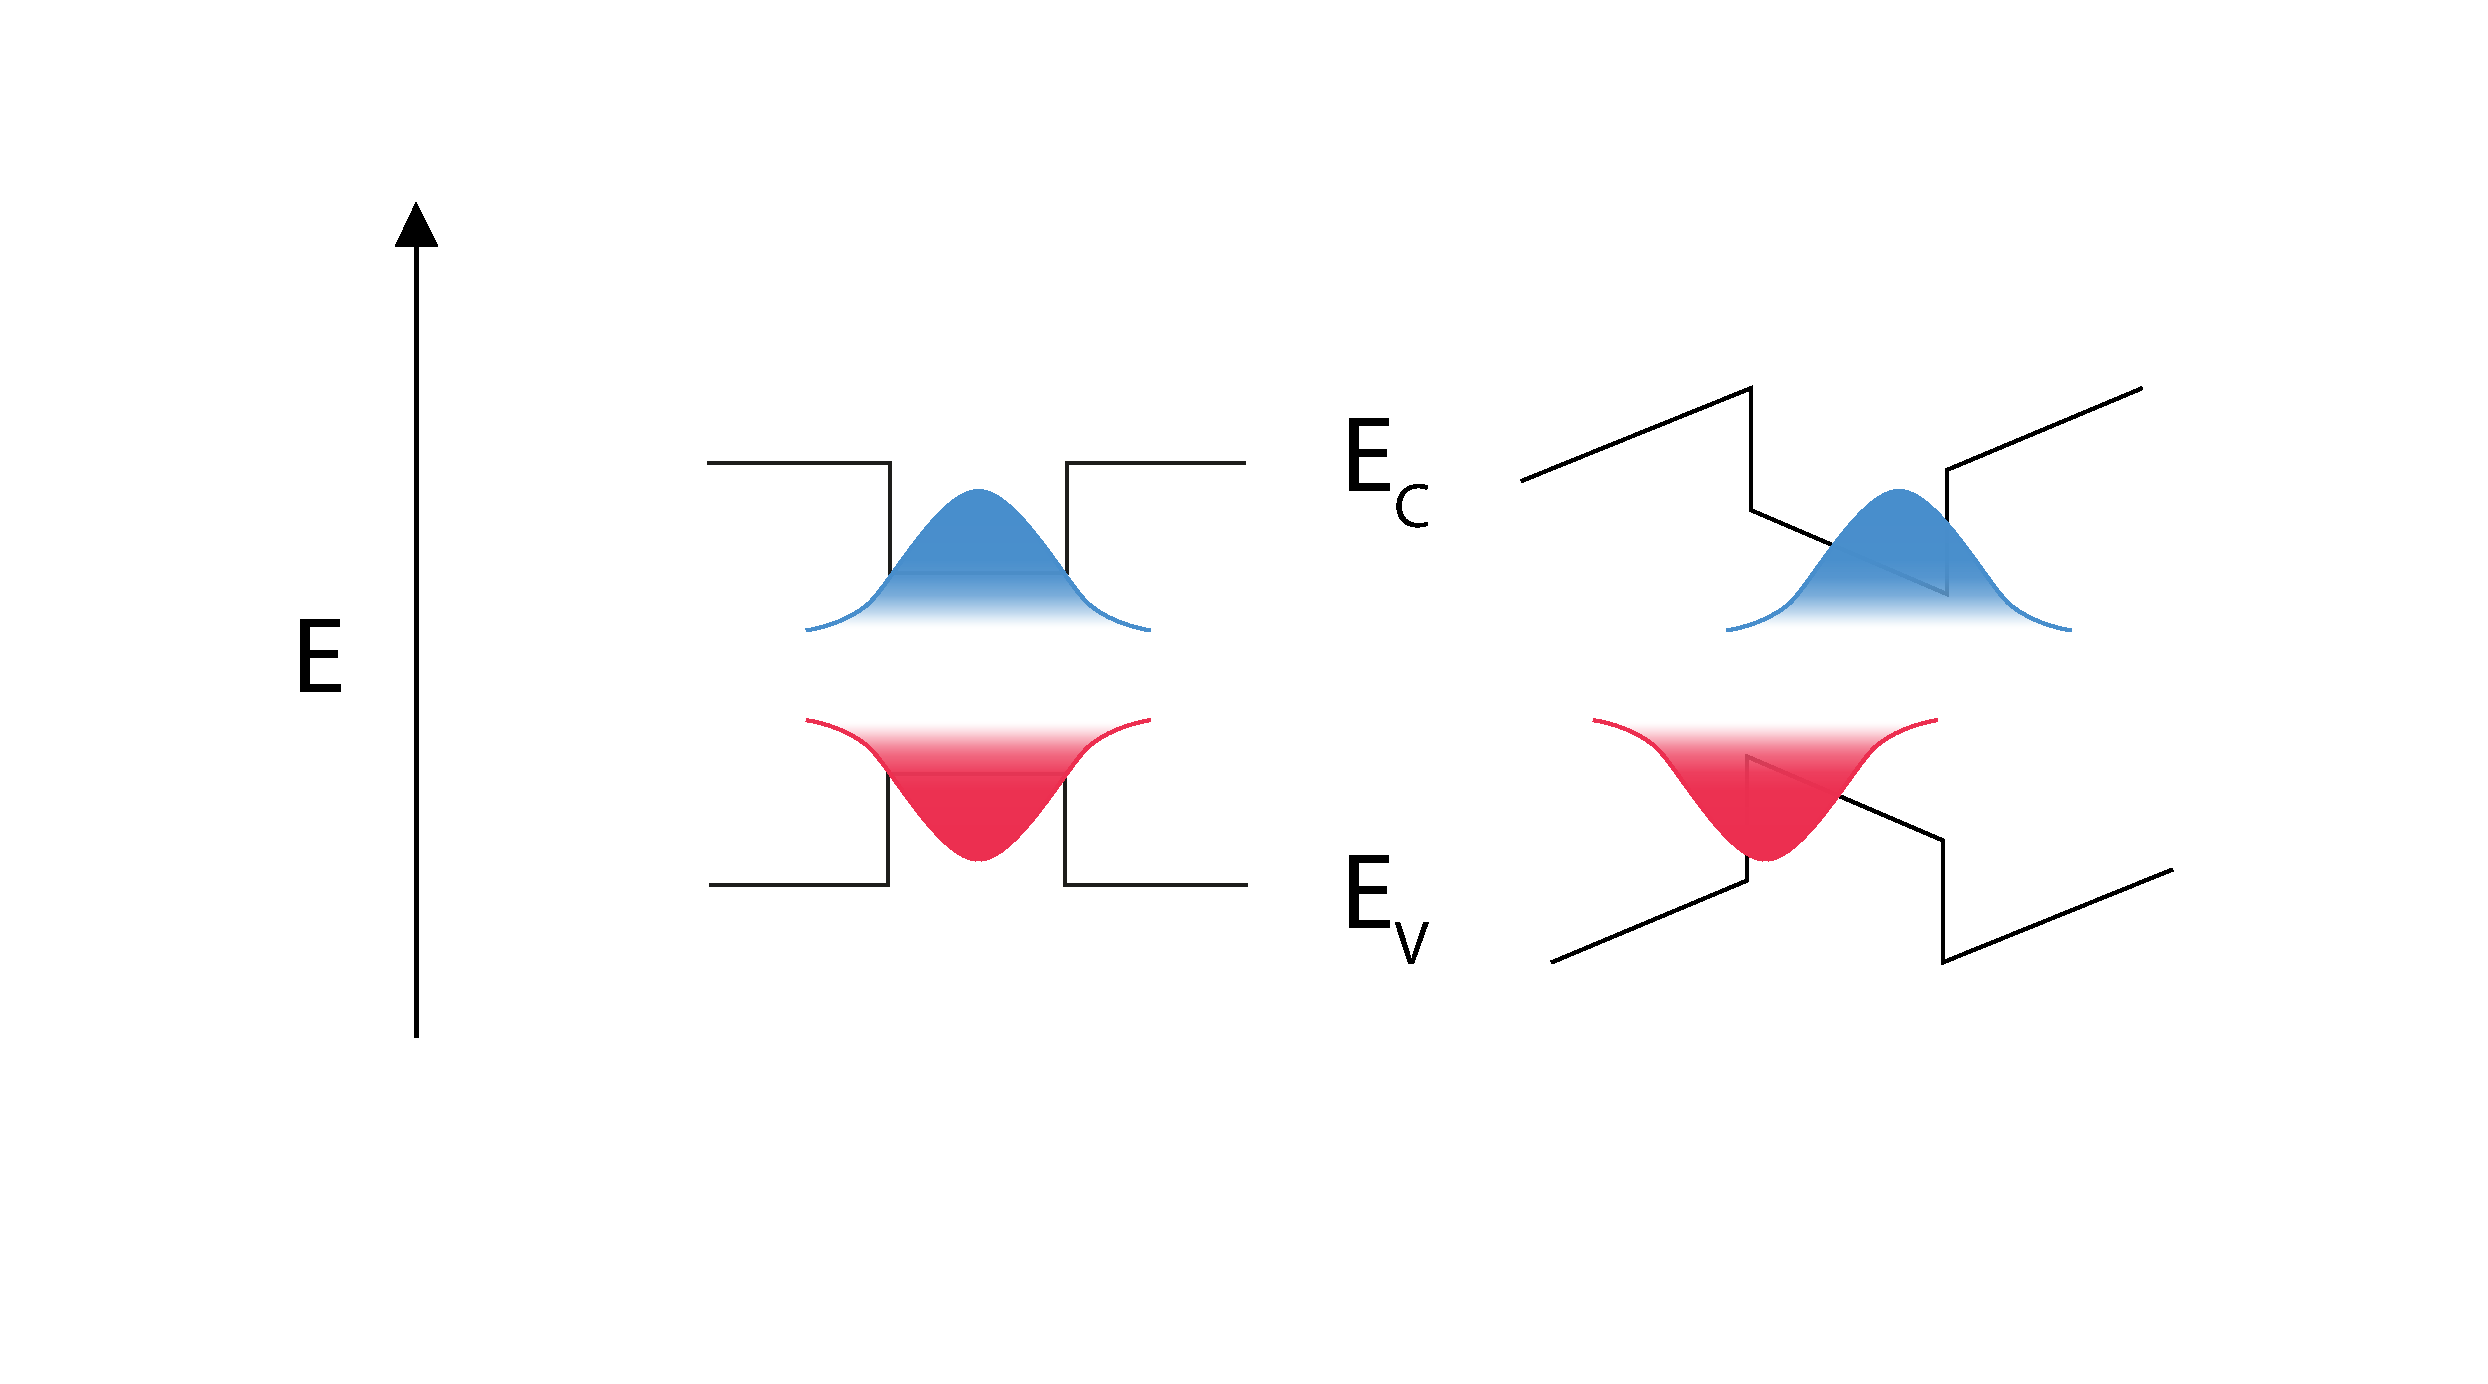
\includegraphics[width=\linewidth]{Bilder/QCSE.pdf}
        \caption{PL-Spektren der Proben ohne Übergitter}
    \end{minipage}% <- sonst wird hier ein Leerzeichen eingefügt
\end{figure}
\vspace{1cm}
\raggedright
%
Die Ursache für die piezoelektrische Polarisation sind die Verspannungen zwischen den in (0001)-Richtung gewachsenen Schichten welche durch die unterschiedlichen thermischen Ausdehnungskoeffizienten und die Gitterfehlanpassung entstehen. Sie wird berechnet nach: 
%
\begin{equation}
    \vec{P}^{pz} = e \cdot \epsilon
\end{equation}
%